\section{Tests}

Das kontinuierliche Testen und Bewerten aller Einzelkomponenten und Funktionen des Systems ist ein elementarer Entwicklungsbestandteil und teilt den Entwicklungsprozess in unterschiedliche Abschnitte.

Leider hat die aktuell herrschende Covid-19 Pandemie die Erstellung und Durchführung aussagekräftiger Tests erschwert. 

\subsection{Mikrofontest}

Noch vor der eigentlichen Entwicklungsarbeit wurden die zur Verfügung gestellten Einzelkomponenten auf ihre Funktion überprüft. Hierzu wurde der Raspberry Pi mit einem Betriebssystem versehen (Raspberry OS 10) und mit der notwendigen c-Bibliothek versehen BCM 2835 V1.68. Über einfache Jumperkabel wurde jeweils ein zu testendes Mikrofon und ein Abschlussmikrofon an den Raspberry angeschlossen und ein Test durchgeführt. (\autoref{fig:BlockbildMirkoTest}).

\begin{figure}[h]
	\begin{center}
		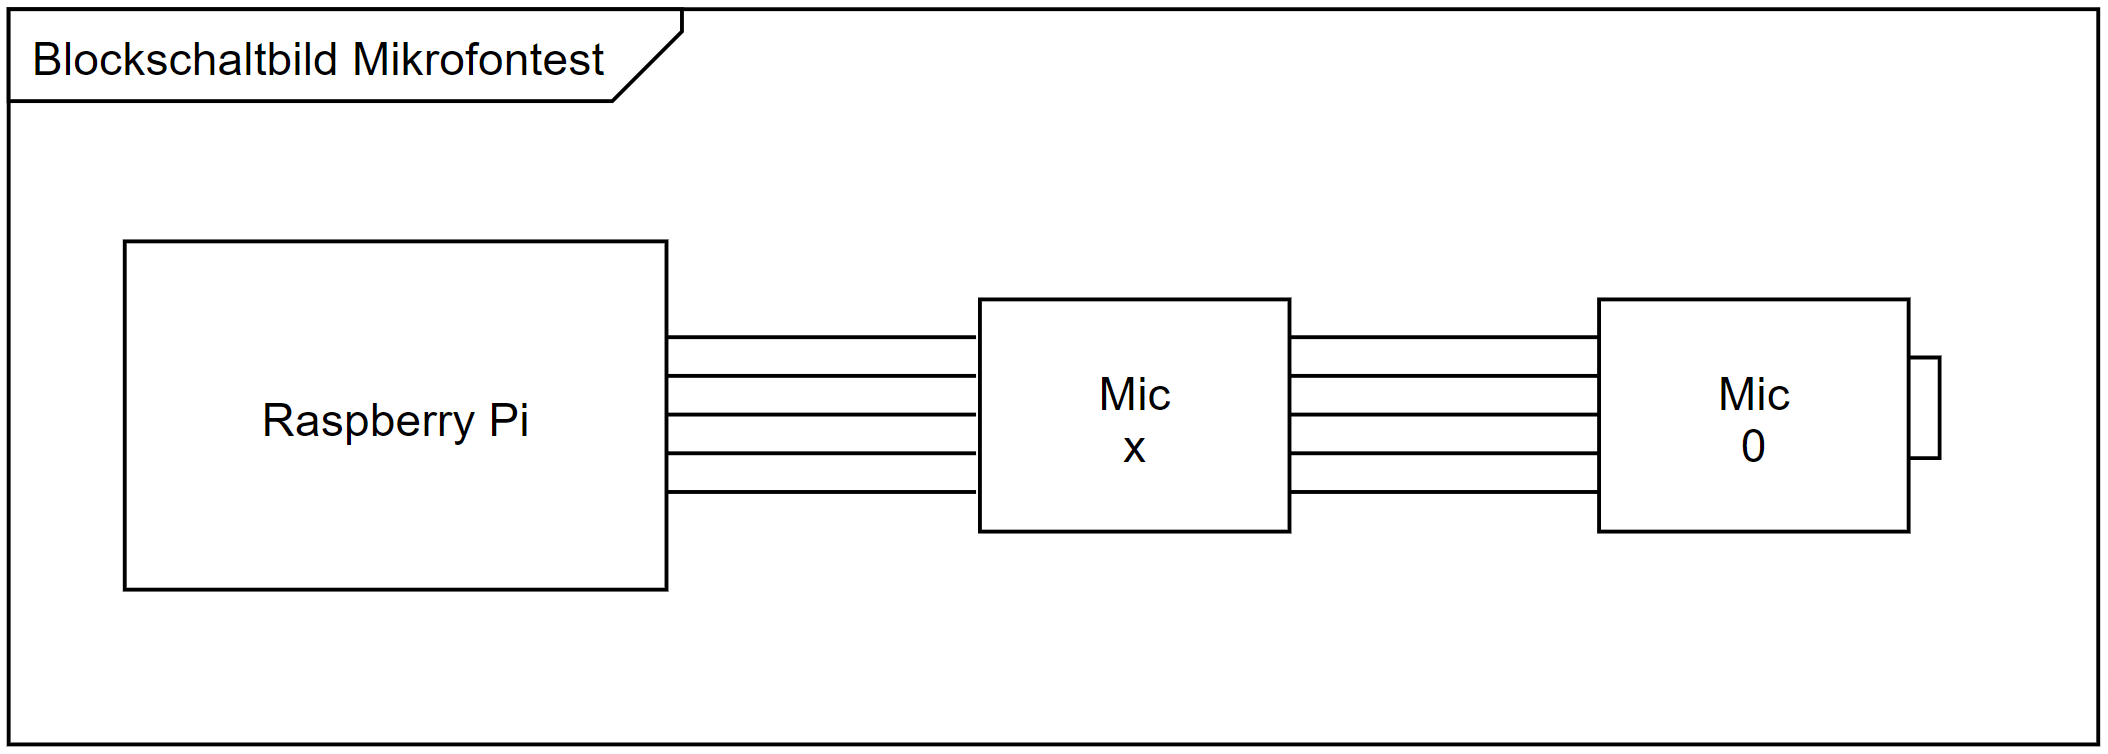
\includegraphics[scale=0.1]{Sections/Tests/BlockbildMikroTest}
	\end{center}
	\caption{Blockbild Mikro Test}
	\label{fig:BlockbildMikroTest}
\end{figure}

Mit dem Skript \glqq RecordMicToRAM\grqq\ wurden die Daten des Mikrofonpaar eingelesen und auf ihre Vollständigkeit überprüft. Es wird eine .txt-Datei erzeugt. In dieser Datei sind 7 Spalten und für das entsprechende Mikrofon tauchen bei erfolgreichem Durchlauf Messwerte auf. So konnte die korrekte Funktion der einzelnen Mikrofone garantiert werden.

\subsection{Hardware Test}

\subsection{Kabelfunktionstest}

In einem ersten Entwicklungsschritt wurde das gesamte Mikrofonarray mit großzügig dimensionierten Verbindungskabeln (Kabellänge ca. 50 cm) aufgebaut und in Abständen von ungefähr \SI{20}{cm} zueinander platziert. 

\begin{figure}[h]
	\begin{center}
		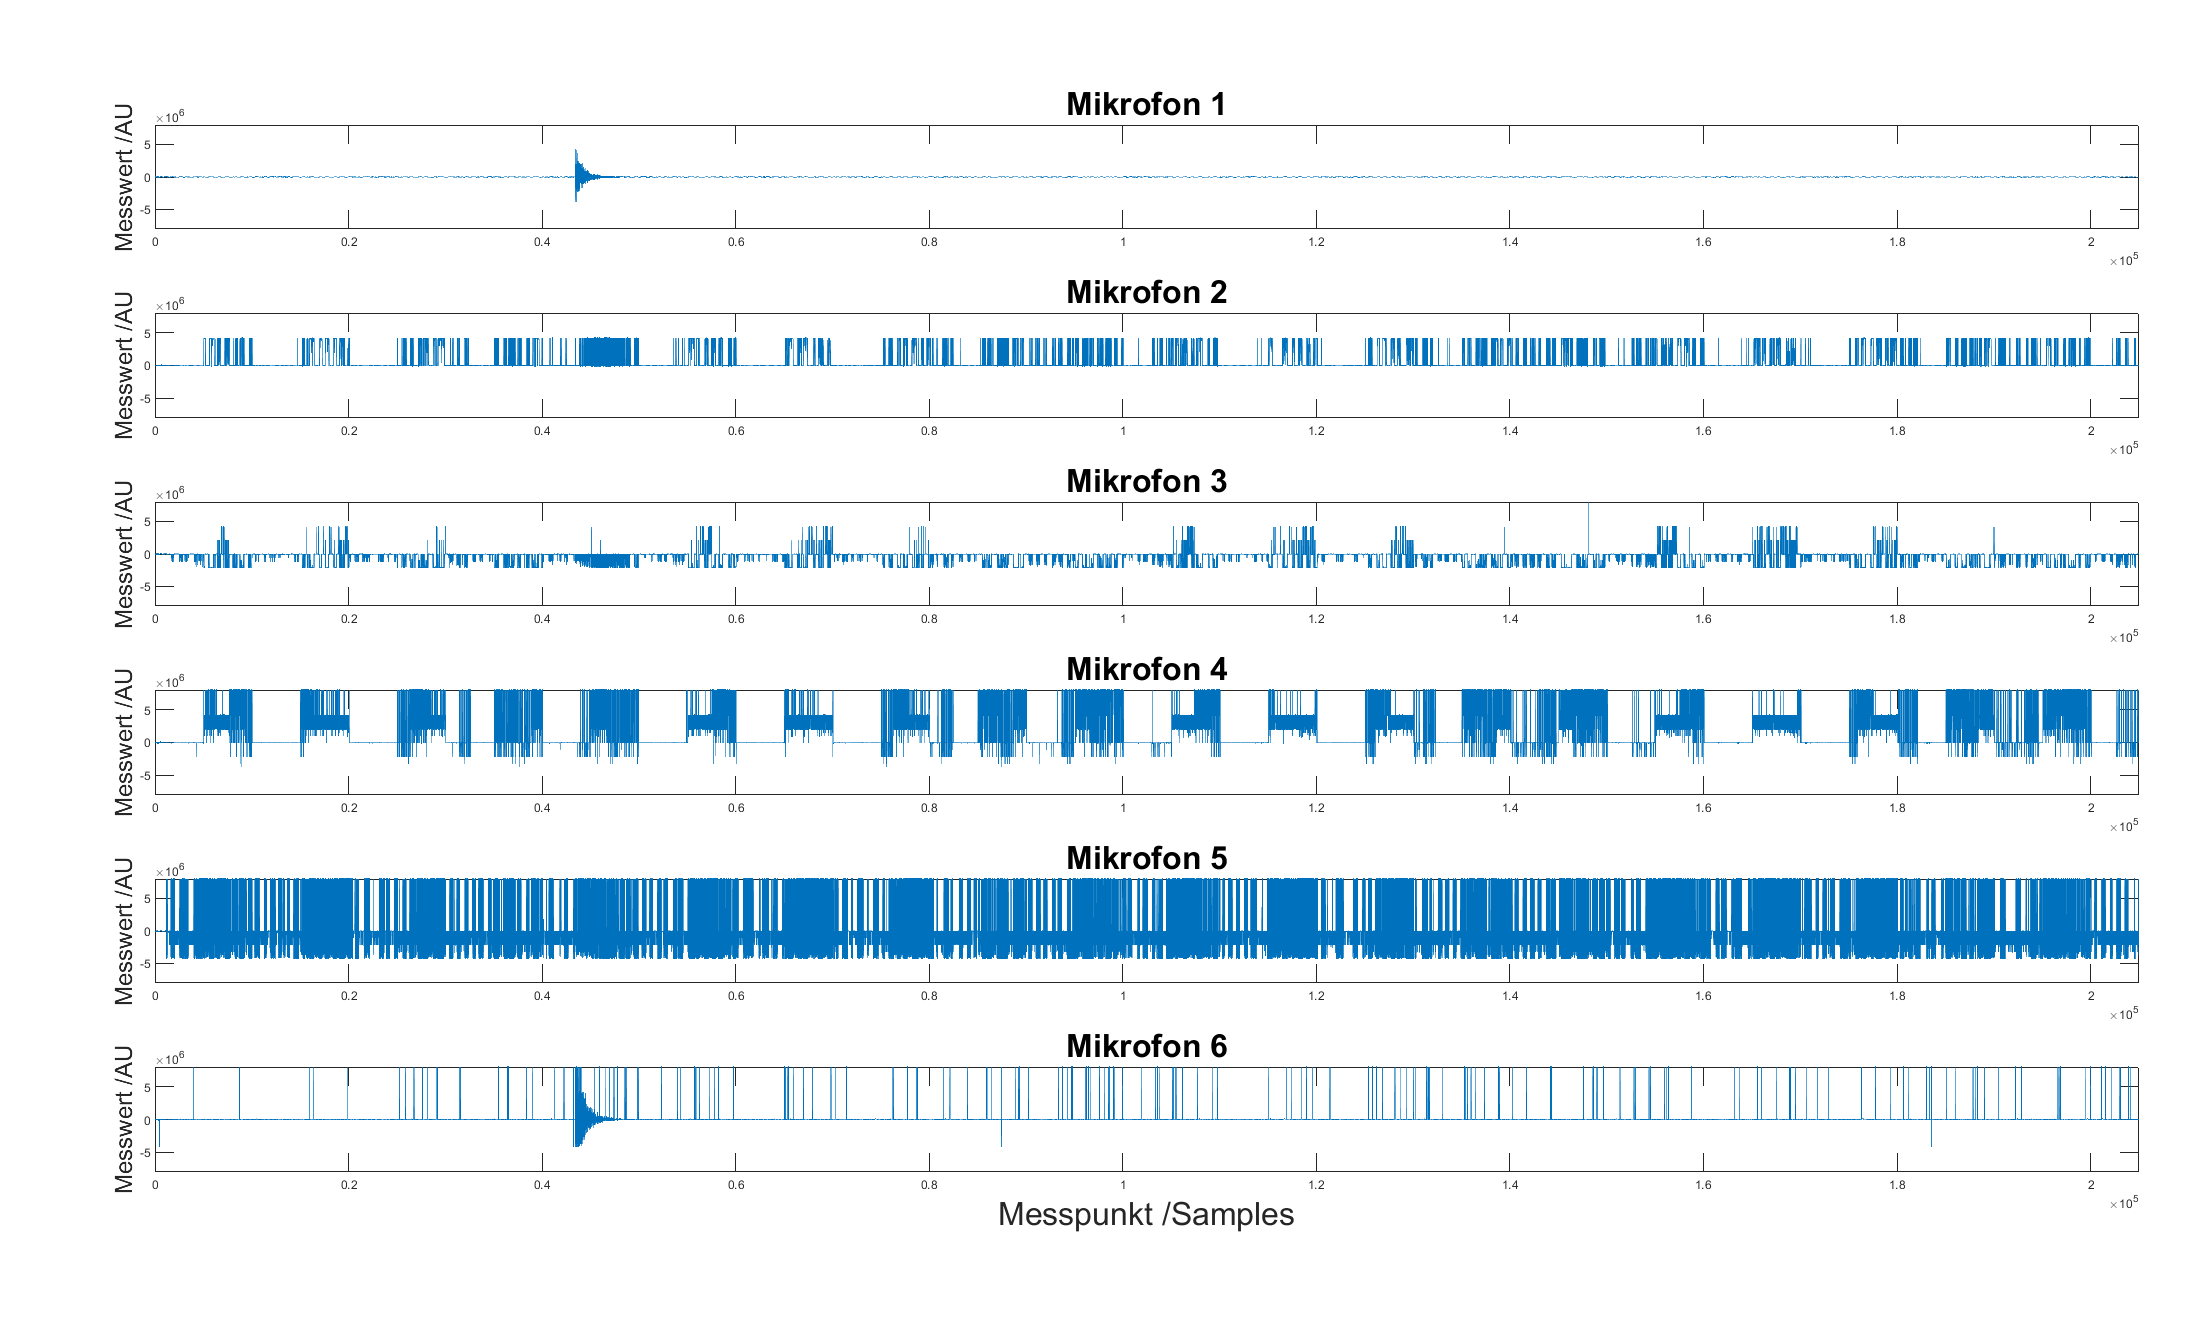
\includegraphics[scale=0.1]{Sections/Tests/Test_1_d}
	\end{center}
	\caption{Kabelfunktionstest 1}
	\label{fig:Test_1_d}
\end{figure}

Die dargestellte Messung wurde über einen Zeitraum von acht Sekunden durchgeführt mit einem Händeklatschen nach ungefähr zwei Sekunden.

Die Erwartungshaltung an die Ergebnisse war ein sauberer Ausschlag der Messwerte bei ungefähr einem Viertel der vergangenen Testzeit mit einem anschließenden Abklingen auf den Umgebungspegel.

Lediglich die Aufzeichnungen aus Mikrofon 1 entsprachen den Erwartungen (Ausschlag bei ca. 40.000 Samples), während die restlichen Mikrofone deutliches Rauschen aufwiesen. In der Aufzeichnung von Mikrofon 3 war selbst das Event (erwartet bei ca. 40.000 Samples) nicht zu erkennen, während auf den anderen Kanälen noch Andeutungen eines stärker verrauschten Bereiches zu erkennen waren. Dieses Verhalten hätte seine Ursache beim Raspberry Pi haben können. Dieser muss für die Taktung der Mikrofone einen SPI-Takt über das gesamte Array treiben können. Mit zunehmender Kabellänge nimmt die Taktsicherheit ab. 

Durch ein Fachgespräch mit Max Weltz schlossen wir auf folgende mögliche Ursachen:

\begin{itemize}
	\item Kabel defekt
	\item SPI-Takt zu hoch
	\item Kabel zu lang
\end{itemize}

Um eine qualitative Ursachensuche vornehmen zu können, beschlossen wir die aufgezählten Ursachen separat zu Untersuchen.

\subsection{Kabelfunktionstest 2}

In einer zweiten Iteration wurde das System umkonfiguriert, sodass jetzt mit einem SPI-Takt von \SI{3,9}{MHz} und nicht wie ursprünglich mit \SI{7,8}{MHz} gearbeitet wird. 

\begin{figure}[h]
	\begin{center}
		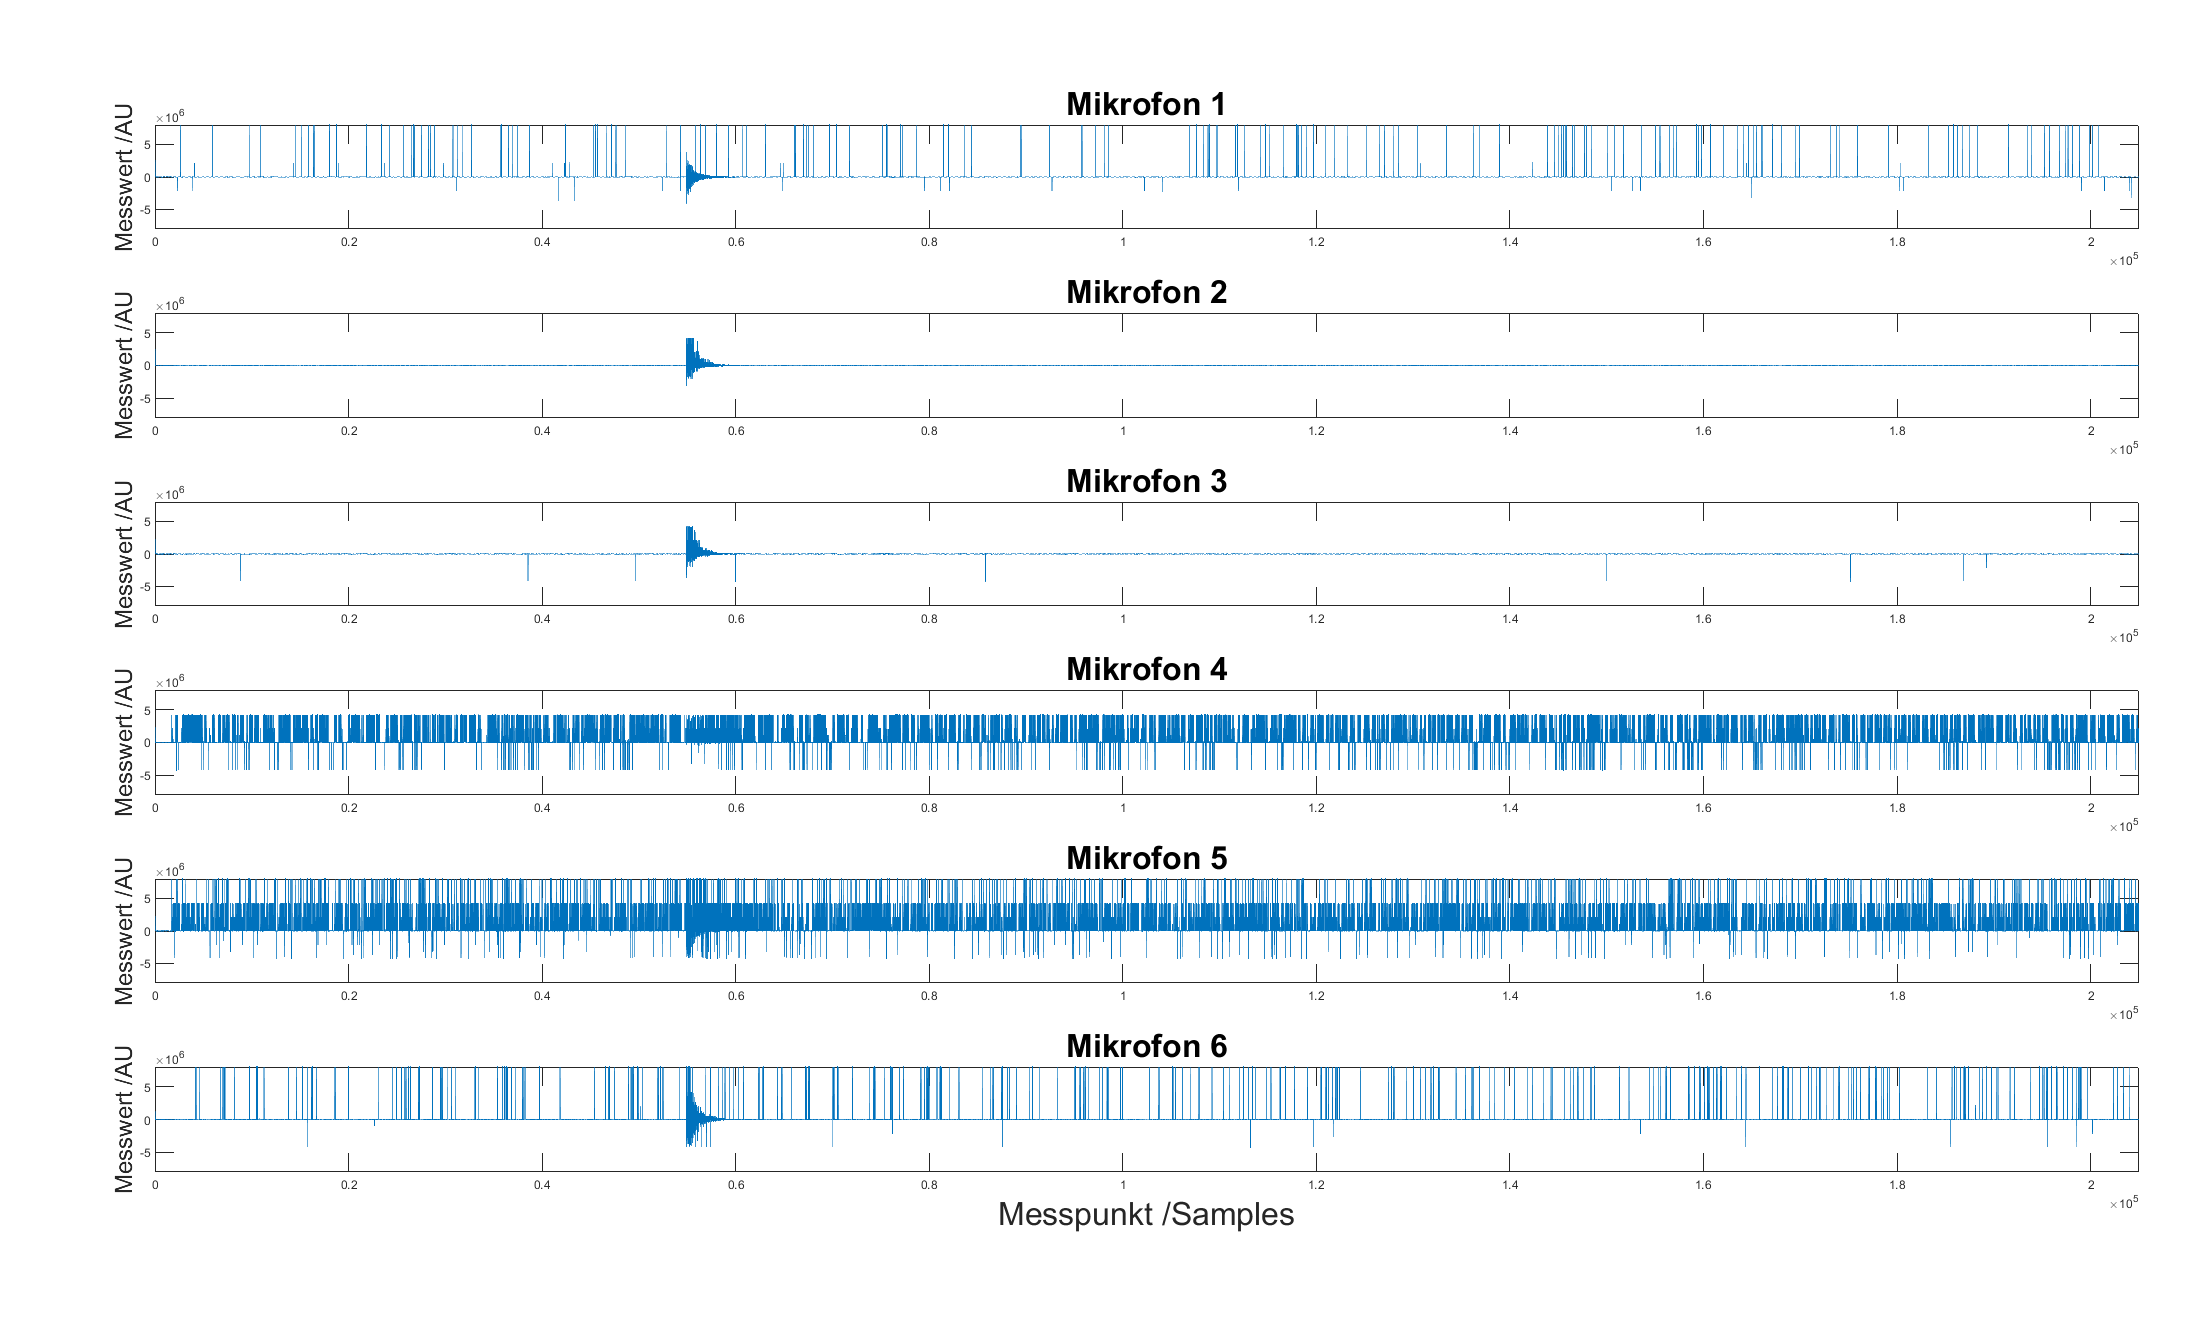
\includegraphics[scale=0.1]{Sections/Tests/Test_2_d}
	\end{center}
	\caption{Kabelfunktionstest 2}
	\label{fig:Test_2_d}
\end{figure}

Für diese Konfiguration wurde die gleiche Testmethode verwendet und es ist zu erkennen, dass die Messungen nun deutlich weniger verrauscht waren. Dennoch sind immer wieder bit-shift Fehler zu erkennen, die das Messergebnis zu bestimmten Schwellenwerten springen lässt. Die Messungen waren somit immer noch zu stark verrauscht und für eine Verwendung unbrauchbar. 

Eine reine Reduzierung des verwendeten SPI-Takts hat das Problem also noch nicht vollständig gelöst.

\subsection{Kabelfunktionstest 3}

In der nächsten Anpassung wurde die Kabellänge der Mikrofonkabel auf nun ca. \SI{25}{cm} reduziert mit der Erwartung, dass die Taktsicherheit über die gesamte Kabellänge steigen sollte.

\begin{figure}[h]
	\begin{center}
		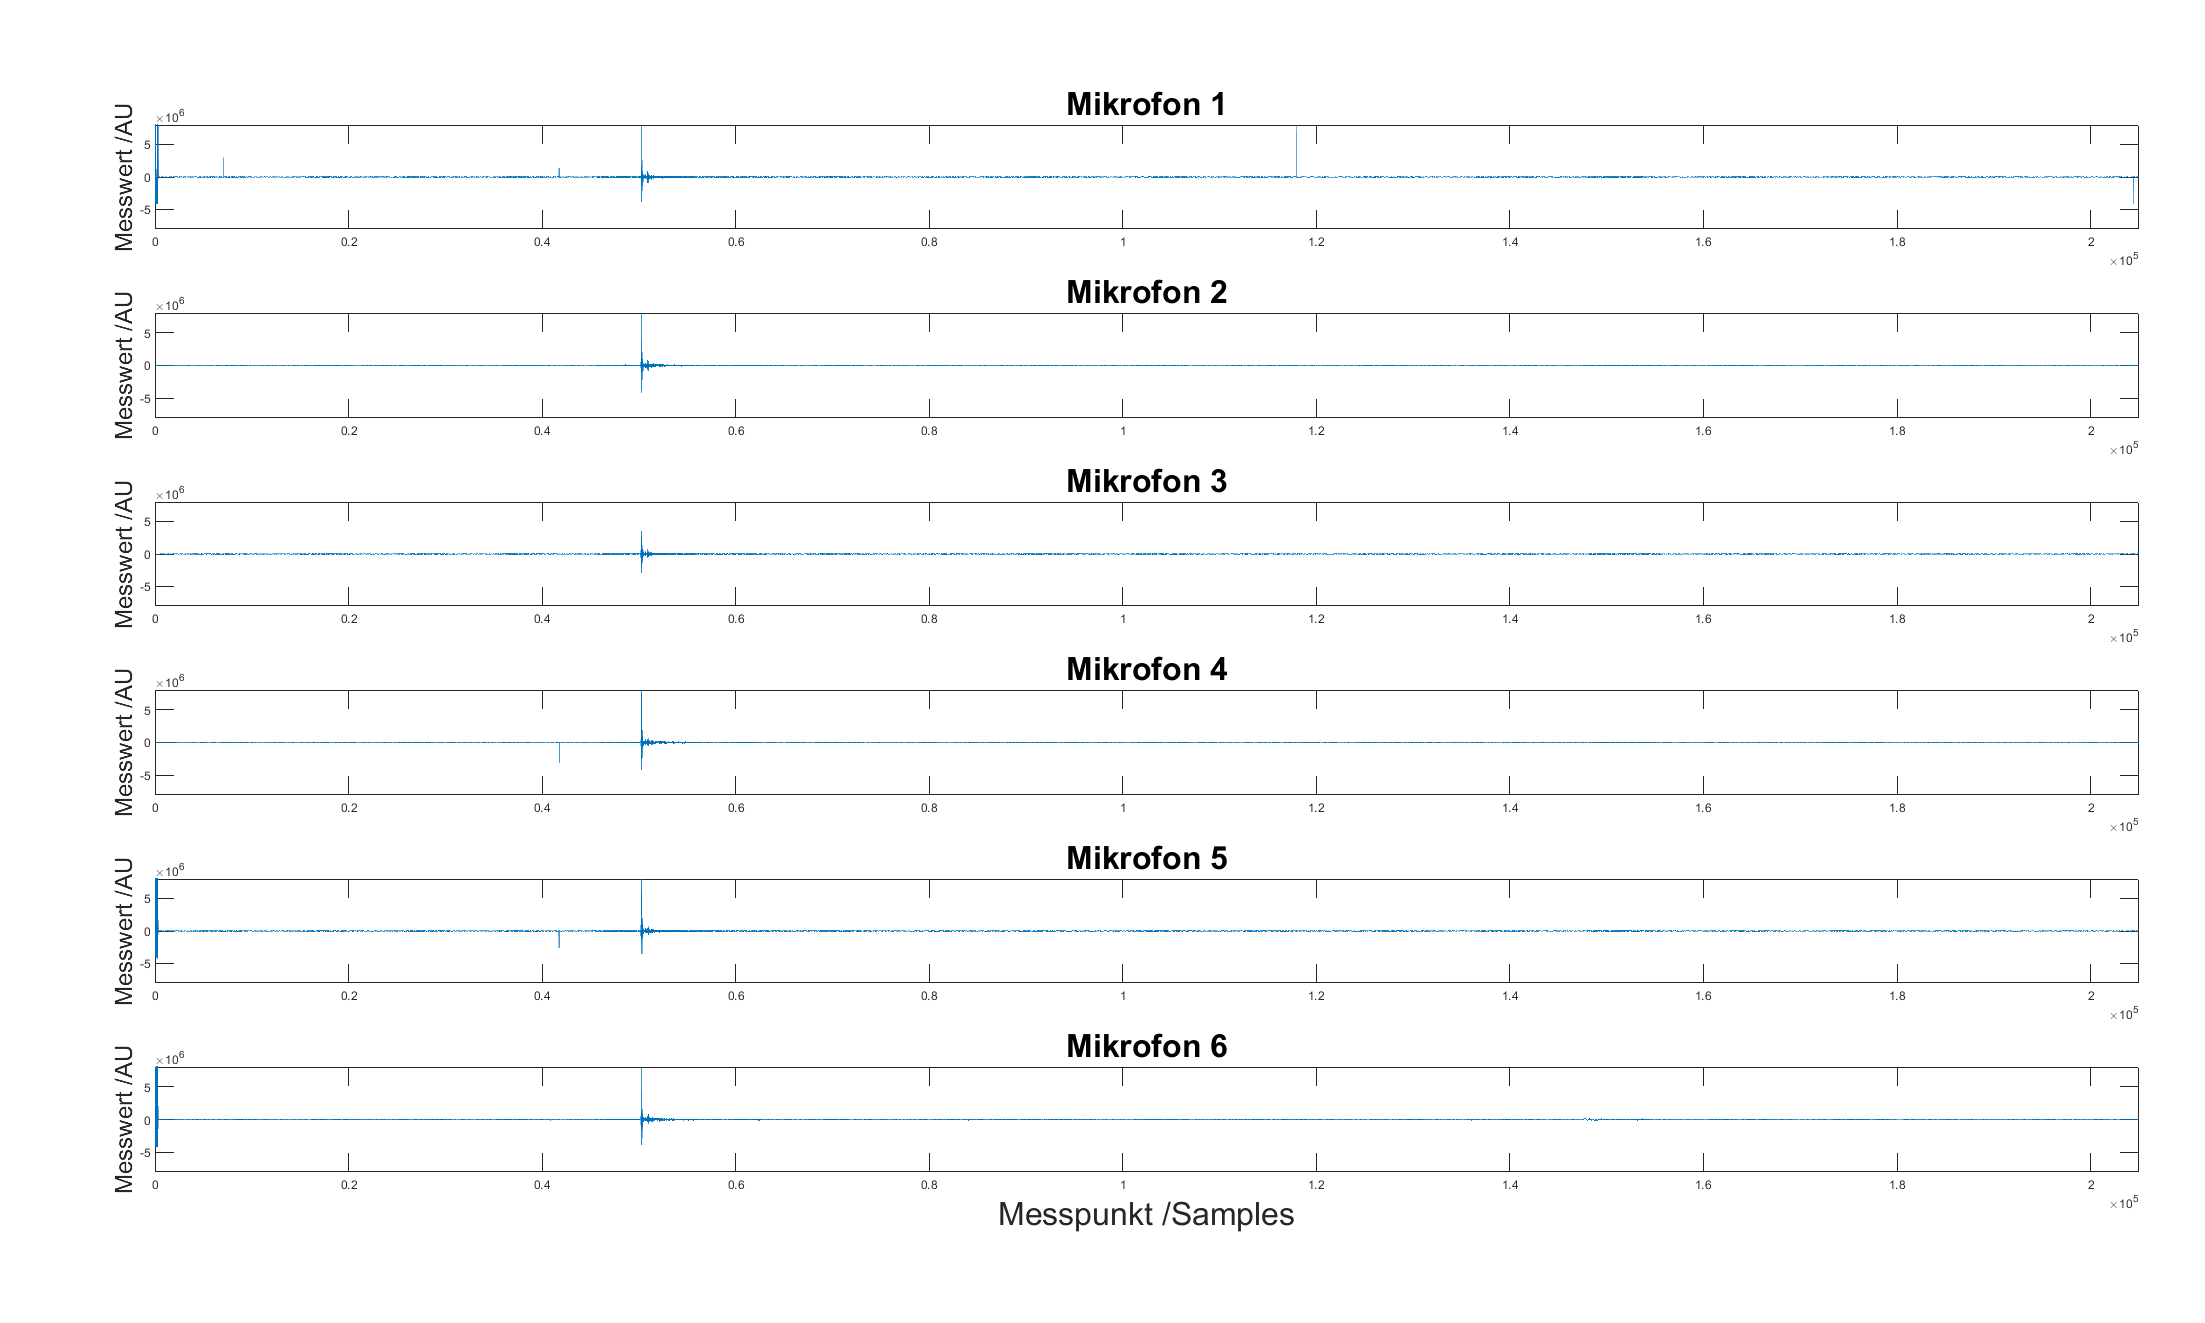
\includegraphics[scale=0.1]{Sections/Tests/Test_3_d}
	\end{center}
	\caption{Kabelfunktionstest 3}
	\label{fig:Test_3_d}
\end{figure}

Die nun durchgeführte Messung wies das gewünschte, rauschfreie Verhalten der Messwerte auf allen Kanälen auf. Die Kabel wurden somit in Bezug auf die Datenübertragung hinreichend auf die Funktion überprüft. 


\newpage